\def\year{2020}\relax
\documentclass[letterpaper]{article} % DO NOT CHANGE THIS
\usepackage{aaai20}  % DO NOT CHANGE THIS
\usepackage{times}  % DO NOT CHANGE THIS
\usepackage{helvet} % DO NOT CHANGE THIS
\usepackage{courier}  % DO NOT CHANGE THIS
\usepackage[hyphens]{url}  % DO NOT CHANGE THIS
\usepackage{amsthm}
\usepackage{amsmath,amssymb}\usepackage{graphicx} % DO NOT CHANGE THIS
\urlstyle{rm} % DO NOT CHANGE THIS
\def\UrlFont{\rm}  % DO NOT CHANGE THIS
\usepackage{graphicx}  % DO NOT CHANGE THIS
\frenchspacing  % DO NOT CHANGE THIS
\setlength{\pdfpagewidth}{8.5in}  % DO NOT CHANGE THIS
\setlength{\pdfpageheight}{11in}  % DO NOT CHANGE THIS
\newcommand{\citename}[1]{\citeauthor{#1}~\shortcite{#1}}
\DeclareMathOperator{\argmax}{argmax}
\DeclareMathOperator{\argmin}{argmin}



\setcounter{secnumdepth}{2} %May be changed to 1 or 2 if section numbers are desired.

\setlength\titlebox{2.5in} % If your paper contains an overfull \vbox too high warning at the beginning of the document, use this
\title{Interpretable Models of Human Interaction in Immersive Simulation Settings}
\author{Paper ID 134 (this is the rejected AAAI paper)}


\newcount\Comments  % 0 suppresses notes to selves in text
\Comments=1

\usepackage{xcolor}
\newcommand{\kibitz}[2]{\ifnum\Comments=1{\textcolor{#1}{#2}}\fi}
\newcommand{\nh}[1]{\kibitz{blue}{[NH:#1]}}
\newcommand{\kg}[1]{\kibitz{red}{[KG:#1]}}
\newcommand{\bjg}[1]{\kibitz{purple}{[BG:#1]}}

\begin{document}

\maketitle


\begin{abstract}
Immersive simulations are increasingly used for teaching and training in many societally important arenas including healthcare, disaster response and science education.
The interactions of participants in such settings lead to a complex array of emergent  outcomes that present challenges for analysis.
This paper studies a central element of such an analysis, namely the interpretability of models for inferring structure in time series data.
This problem is explored in the context of modeling student interactions in an immersive ecological-system simulation.
Unsupervised machine learning is applied to data on system dynamics with the aim of helping teachers determine the effects of students' actions on these dynamics.
We address the question of choosing the optimal machine learning model, considering both statistical information criteria and interpretabilty quality.
Our approach adapts two interpretability tests from the literature that measure the agreement between the model output and human judgment.
The results of a user study show that the models that are  the best understood by  people are not those that optimize information theoretic criteria.
In addition, a model using a fully Bayesian approach performed well on both statistical measures and on human-subject tests of interpretabilty, making it a good candidate for automated model selection that does not require human-in-the-loop evaluation.
The results from this paper are already being used in the classroom and can inform the design of interpretable models for a broad range of socially relevant domains.
\end{abstract}



\section{Introduction}
\label{sec:introduction}
There is increasing evidence of the value of multi-person embodied simulations for engaging learners in a variety of
applications, such as healthcare, disaster response and education~\cite{alinier2014immersive,amir2013plan}.
Such simulations involve multiple participants simultaneously executing actions that change the state of the simulated world, emulating the social aspect of these problem domains~\cite{smordal2012hybrid}.

For example, consider Connected Worlds\footnote{\url{https://nysci.org/home/exhibits/connected-worlds/}},  the system studied in this paper. Connected Worlds is
an immersive mixed-reality learning environment
where students interact with an ecological simulation and learn about the causal effects of their actions over time~\cite{mallavarapu2019connect}.
Students' actions have both immediate and long-term effects on the simulation leading to a rich array of emergent outcomes which engender diverse opportunities for learning.
We use Connected Worlds as it provides a good example of an immersive simulation where the simultaneous actions of participants result in complex responses from the system.

Participants in immersive simulations (both instructors and trainees) need to understand how the aggregation of the trainees' individual actions affect the system dynamics over time.
However, no one person can possibly follow what happens, even in a relatively short simulation.
To provide adequate support for participants, AI systems need to consider not just how well they model the data (e.g., log-likelihood), but also how well people understand the representations that are induced by the models that they employ.

This paper studies the \emph{interpretability problem}: determining the AI model (from a set of candidates) that produces the output that is  best understood by people when it is presented  to them~\cite{gilpin2018explaining,doshi2017roadmap,caruana2015intelligible}.
We explore a trade-off between the selection of models in an offline manner, to optimize a log-likelihood objective, and the selection of models that maximise an intrepretability score, that is operationalized via experimental tests with people.

The approach consists of the following:
(1) choosing a set of models for describing the effects of participants' activities in the simulation;
(2) designing tests for computing the interpretability score of a given model applied to Connected Worlds data, based on the agreement between the model output and human judgement; and
(3) comparing the models selected under statistical measures to the models that are selected to maximise the interpretability score.


We use hidden Markov models (HMMs) to model the system dynamics, with an additional set of ``sticky'' hyperparemeters which bias the transition dynamics of the latent state space~\cite{fox2008hdp}.
The input to each model is a multidimensional time series representing the system's responses to students' activities.
The output of the model is a segmentation of the time series into a set of periods, which are contiguous lengths of time during which the system
dynamics are stable (as judged by the model). Each period thus corresponds to a latent state which persists through time.





We applied two interpretability tests to our setting, namely the Forward Simulation and Binary Forced Choice tests~\cite{doshi2017roadmap}.
The tests visualized a model's output by presenting to people images of the simulation that correspond to periods inferred by the model.

We compared the interpretability score %, as evaluated by a user study,
of a variety of models by exploring the space of hyperparameter settings.
One of the models, the fully Bayesian model, does not set the value for the hyperparameters but rather treats them as unknown and stochastic variables in the model by placing priors over the hyperparameters.
This model does not require the explicit choice of values of the hyperparameters of interest.

Our scientific hypotheses were that 1) varying the bias hyperparameters of a model would affect its interpretability; and 2) there exists a setting for the bias hyperparameters that would induce an optimally interpretable model.


The results confirmed Hypothesis 1: there was a variance in model interpretability induced by varying the model hyperparameters.
In particular, the model that optimized the information criteria did not correspond to the optimally interpretable model according to the interpretability tests.

Hypothesis 2 was partly confirmed, in that there was a region in parameter space that induced higher interpretability scores. We were not able to identify a single parameter setting that was the most interpretable setting.
The fully Bayesian approach, which does not require any hyperparameter tuning, provided a good balance between interpretability and performance on the theoretical statistical tests.
We argue that this approach can be suitable for situations in which human evaluation testing is infeasible, unethical or impractical.




In studying the interpretability problem applied to a socially relevant class of domains, that of students' interactions in immersive simulation, we make two contributions to the field.
First, we operationalize two interpretability tests and apply them to real-world data.
Second, we show that the fully Bayesian solution shows promise for model selection when access to human experimentation is infeasible.

The results from this work have already been implemented in a classroom experiment where visualizations of the model's output were shown to the school students who participated with the immersive simulation. The students used the visualizations to bolster their interpretations of events that occurred.
















\section{Related Work}

This paper relates to a burgeoning body of work on evaluating the interpretablity of machine learning models using human judgment~\cite{rosenfeld2019explainability,gilpin2018explaining,doshi2017roadmap,weller2017challenges}.
\citename{doshi2017roadmap} suggested three   tests to evaluate how interpretable a model's representations are to people.
Forward Simulation: requires the evaluator to predict the output of a model for a given input.
Binary Forced Choice: requires the evaluator to choose one of two plausible model explanations for a data instance.
Counterfactual Simulation: requires the evaluator to identify what must be changed in an explanation to correct it for a given data instance.

In follow-up work~\citename{lage2018human} propose a model selection process that considers both a model's accuracy and its degree of interpretability, given by one of the above tests.
They provide a framework for iteratively optimizing the interpretability of a model with a human-in-the-loop optimization procedure. Their work applied this framework to a test setting in the lab in which human judgment was used to optimize supervised learning models.
Other works that studied interpretability tests for supervised learning settings include~\citename{wu2018beyond,ribeiro2016should,choi2016retain,lipton2016mythos}.

We extend this literature on interpretability in several ways.
First, by adapting the model selection process to an unsupervised learning setting, that of segmenting a multi-dimensional time series into periods.
Second, by designing specific Forward Simulation and Binary Forced Choice tests that can be applied to data from a real-world immersive simulation.

Our work was  inspired by \citename{chang2009reading} who were the first to show that optimizing machine learning models in unsupervised settings using predictive log-likelihood may not induce models that are coherent for people.
They focused on the use of topic models for finding meaningful structure in documents and they compared the models that are selected to optimize \textit{perplexity} (analogous to held-out log-likelihood) to the models that were selected by the human interpretability tests that they designed.


\citename{chang2009reading} operationalized two Forward Simulation tests for evaluating the interpretability of a topic model: word intrusion, in which the evaluator is required to identify which of several words does not belong together in one topic represented by the other words; and  topic intrusion, in which the evaluator is required to
identify which of several topics is not associated with a given document.
We extend this work
to a multi-dimenstional time series domain and we introduce a Binary Forced Choice test to complement the ``intrusion'' Forward Simulation test.
















\begin{figure}[t]
\centering
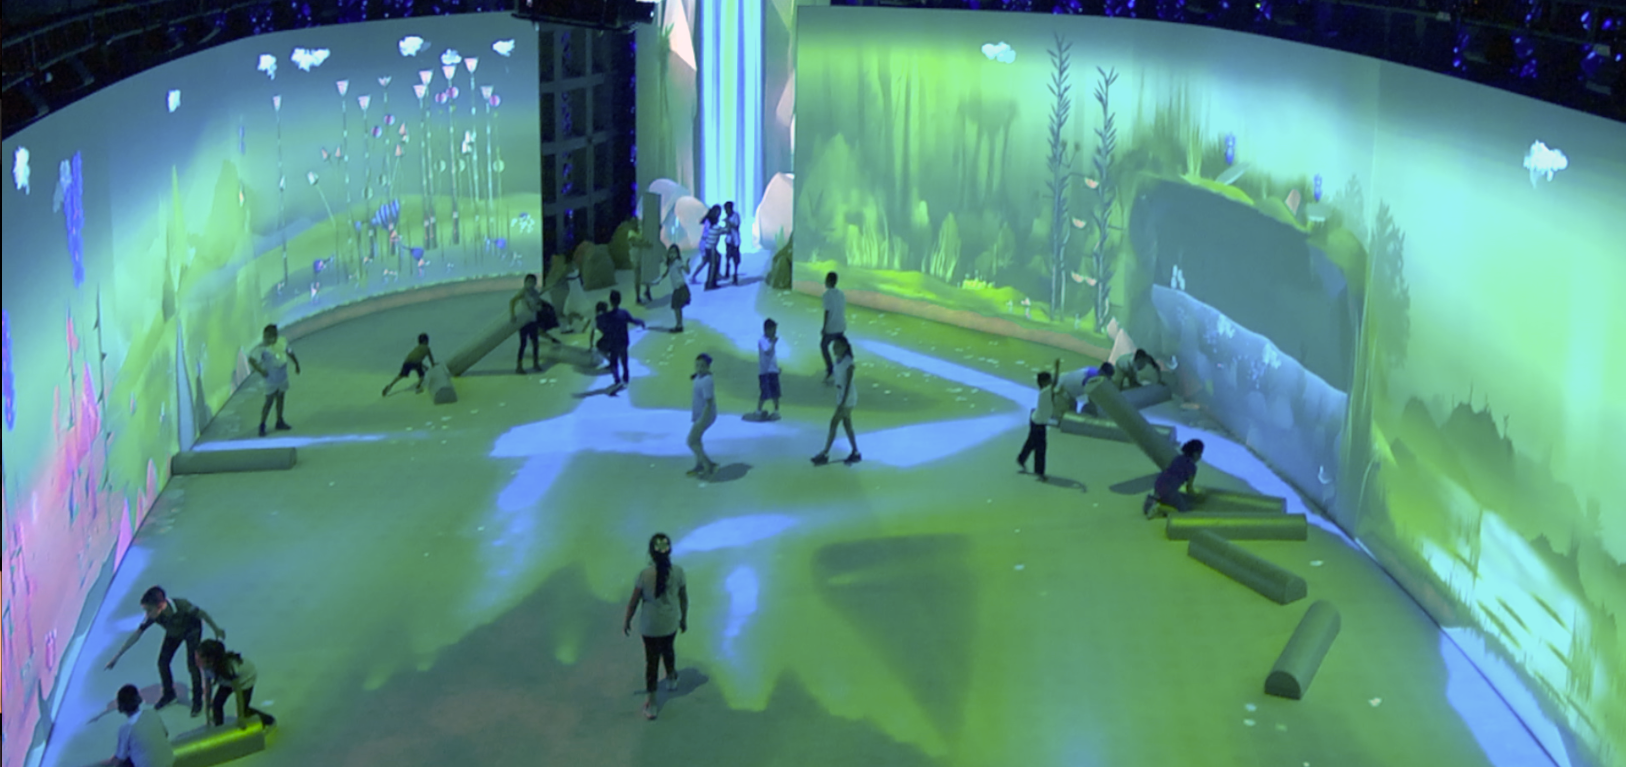
\includegraphics[width=0.48\textwidth]{./images/cw_viz2.png}
\caption{Picture of the floor of Connected Worlds; facing the Waterfall from the area labelled ``Floor'' in Figure~\ref{fig:connected_worlds_graphic}.}
\label{fig:connected_worlds_viz}
\end{figure}


\section{The Connected Worlds Domain}
\label{sec:cw_desc}
Connected Worlds (CW) is a multi-person ecology simulation (installed at a science museum that hosts classes on field trips,) and has the goal of teaching students about complex systems and systems thinking.
It is an immersive environment-simulation comprising four biomes (Desert, Grasslands, Jungle \& Wetlands) that are connected by a central flow of water, fed by a waterfall. The simulation exhibits large scale feedback loops and presents the opportunity for participants to experience how their actions can have (often unintended) effects that are significantly removed in time and/or space. Students plant trees which flourish or die, animals arrive or depart, and rain clouds form, move through the sky and deposit rain into the waterfall.
Figure~\ref{fig:connected_worlds_viz} shows a photograph of the CW space where participants are seen to be interacting with both physical and virtual objects in the simulation.

Students interact with CW by physically moving plush logs to control the direction of water that flows in the simulation. Water can be directed to each of the four biomes and the distribution of flowing water depends on the placement of the logs. Water enters the simulation via rainfall events which are out of the students' control. These release water into the waterfall (to replenish the primary source of water) and into the individual biomes.

\begin{figure}[t]
\centering
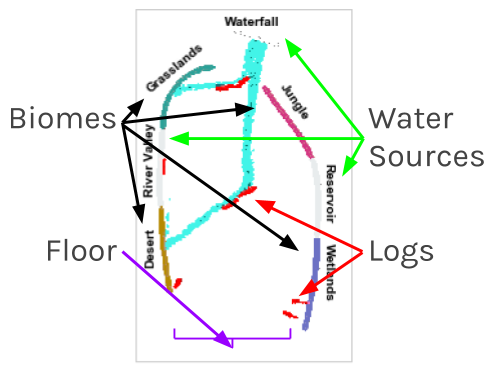
\includegraphics[width=0.48\textwidth]{./images/cw_snapshot.png}
\caption{CW snapshot view. Biomes are labelled on the perimeter and logs appear as thick red lines. Water (blue stream in the middle of the image) enters via the waterfall and in this image it mainly flows toward the Grasslands and the Desert.}
\label{fig:connected_worlds_graphic}
\end{figure}

The nature of the simulation is complex on a variety of dimensions as it involves a large number of students simultaneously executing actions that change the state of the simulated environment. Thus, each participant will have a different view of what transpired, depending on the actions s/he took and the state changes that resulted.
It is therefore important to develop tools that can support  the understanding of the students' interactions in complex environments such as CW.
Such tools can  support teachers and students in reflecting upon and generalizing from their simulation experience.

A data set ($D$) consists of 8-minute long sessions where students interact with CW.
For each session, the system logs the water levels in the simulation at a 1Hz frequency, forming a time series that describes the effects of the students' actions on the water flow in the simulation.
CW also provides
a visual representation of the system state, referred to as the \emph{session view}; a snapshot from this representation is shown in Figure~\ref{fig:connected_worlds_graphic}.
We use two controlled sessions of students interactions with CW.\footnote{Access to the data files is currently restricted but can be granted upon request.}\footnote{We followed an approved IRB protocol for the collection of our data.}







\section{Measuring Interpretability}
\label{sec:interpretability_tests}

\begin{figure}
\centering
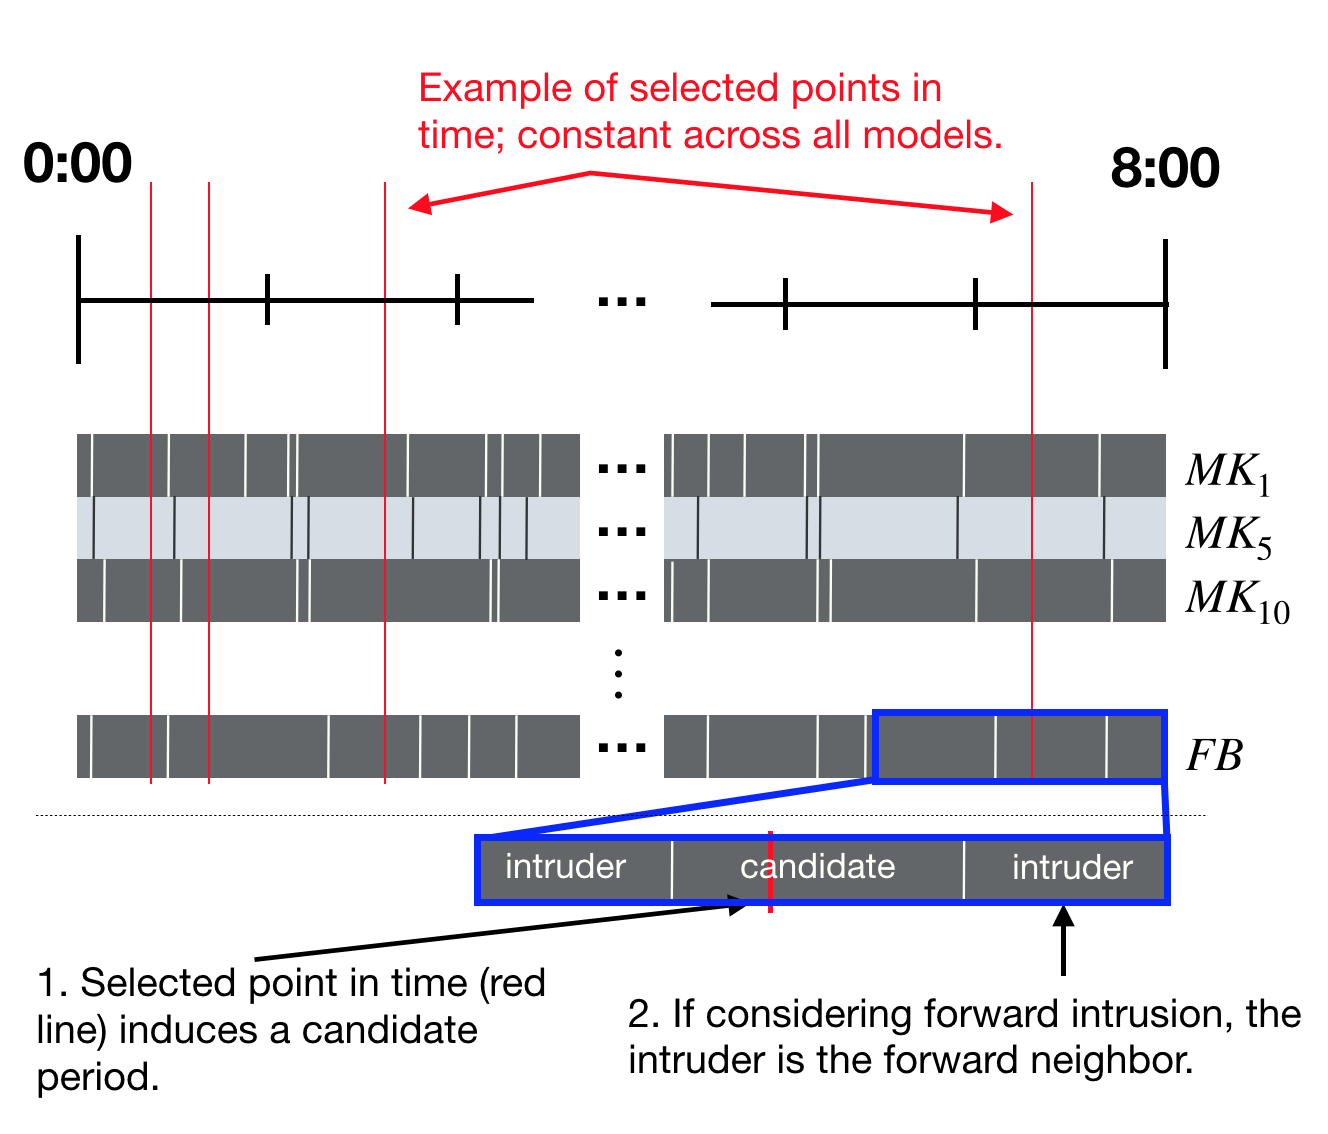
\includegraphics[width=0.45\textwidth]{images/period_selection_representation}
\caption{
\textbf{Top:} segmenting a time series into periods. The data series is represented as a horizontal line from minute 0 to 8; red vertical lines denote sampled time points in the time series; each model is shown as a grey rectangle; models segment time series into periods delimited by white vertical lines. \textbf{Bottom:} the forward or backward neighbour of the candidate period is selected as an intruder.}
\label{fig:selection_representation}
\end{figure}

\begin{figure*}[t]
\centering
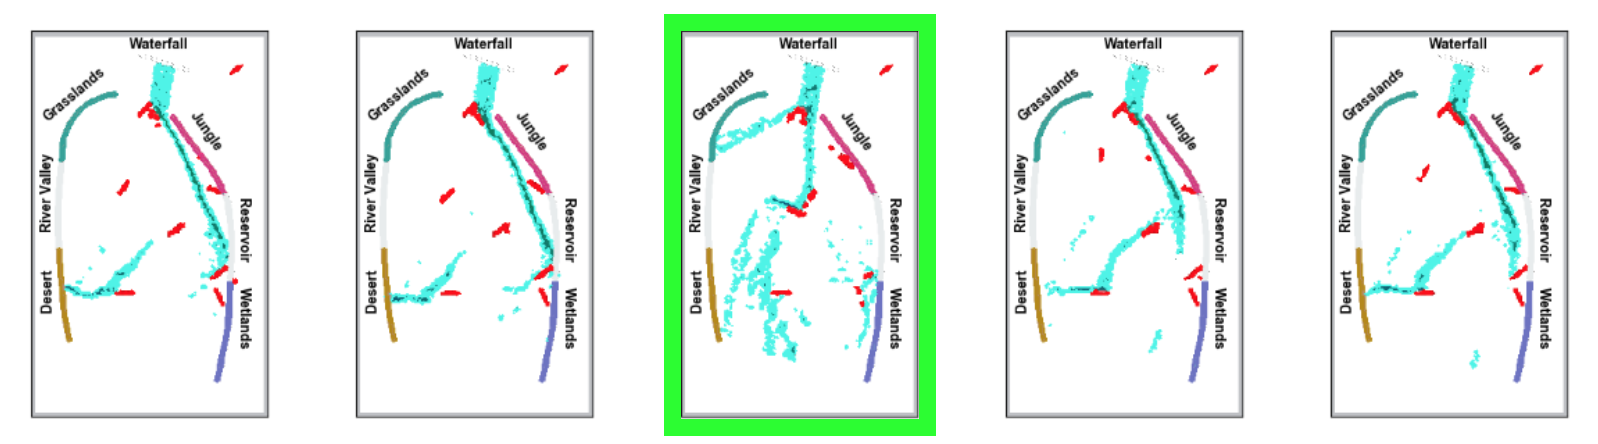
\includegraphics[width=0.75\textwidth]{images/test1_screenshot}
\caption{Screenshot of the  Forward Simulation  test interface. Here $4$ of the images show water flowing towards the Wetlands with a small stream being directed to the Desert. An intruder image, the highlighted one, shows water flowing to the Grasslands and there is neither water flowing to the Wetlands nor to the Desert in this image.}
\label{fig:test1_screenshot}
\end{figure*}

We use an interpretability score $IS$ to measure the interpretability of a model $M$ applied to a data set $D$ ($IS: M \times D \rightarrow \mathcal{R}$).
The interpretability score is operationalized via an interpretability test which takes as input a model segmentation of a time series (into periods) and a selected point in time $i$ from the time series.
Each test consists of a \emph{visualization} which presents any period as a set of images extracted from the session view.
A test instance returns True if an evaluator successfully completes the required objective. For the   Forward Simulation test, the objective is to correctly simulate the model output for a given instance. For the Binary Forced Choice test, the objective is to correctly  identify the best model output that matches a given instance.




We adapted the Forward Simulation and Binary Forced Choice tests~\cite{doshi2017roadmap} to the CW domain using the notion of \textit{candidate} and \textit{intrusion} periods.
We say that period $p$ is \textbf{active} for model $M$ at time $i$ if  $M$ infers the period $p$ to describe a contiguous length of time in the time series, and $p$ includes the time $i$.
Figure~\ref{fig:selection_representation} shows how a time point (red vertical line) is used to select a candidate period where the candidate period is the active period from model $M$ at $i$ (the active period for a model intersects with the red line).

Hypothetically, the intruder can be any period in a model's segmentation of the time series.
However, intrusion periods that are further away in time from the candidate period would be easier to detect due to the non-stationary evolution of the system.
We make a design decision to chose the period that is immediately adjacent to the candidate period, either forward or backward in time, thereby testing the specific choice of boundary between the two periods.
Figure~\ref{fig:selection_representation} (bottom) shows that the intrusion period is selected as the neighbor to a candidate.


Figure~\ref{fig:test1_screenshot} shows an example of the Forward Simulation test.
This test sampled 4 session-view images from the candidate period of $M$ at $i$, and a single session-view image for the intrusion period.
The images were presented in a random order.
The test evaluator was required to identify which image was the intrusion image.
In Figure~\ref{fig:test1_screenshot}, the image that is outlined in green is the intrusion image that corresponds to the intrusion period.
Since the output of model $M$ is a segmentation of a time series into periods, if the test evaluator could distinguish between the candidate and intrusion periods, this corresponds to them simulating the choice of two of these periods.


Figure~\ref{fig:test2_screenshot} presents an example of the Binary Forced Choice test.
The test displays an unknown session-view image from a candidate period (center of screen) and two competing explanations for this image (``Period 1'' or ``Period 2'').
Each of the  two competing explanations is visualized as four images sampled from the candidate or the intruder period.
The unknown image is sampled in time close to the boundary of when the candidate period transitions into the intruder period (or when the intruder period transitions into the candidate period if the order was reversed).
A test evaluator is required to choose between the two competing explanations.
In Figure~\ref{fig:test2_screenshot}, Period 1, highlighted in green, is the correct choice of explanation for the unknown image.


Given data set $D$ and model $M$, the interpretability score $IS$ of a model is equal to the expectation   of the test over sampled points in a time series $D$.
\begin{equation}
\label{eq:interpretability_score_eq}
IS(M,D) = E_{i\sim D} [ T (M,D,i)]
\end{equation}
Where $T(M,D,i)$  denotes the average test score (over all evaluators) of model $M$ on data set $D$ at sampled point in time $i$. The set of time points $\{i\}$ were uniformly sampled from the time series with the additional constraint that each minute of interaction had at least one sample.
For every model we test, we hold constant the selected times $\{i\}$ in the time series. In this way we  control for different areas in the time series being more or less difficult to segment.




\begin{figure*}[t]
\centering
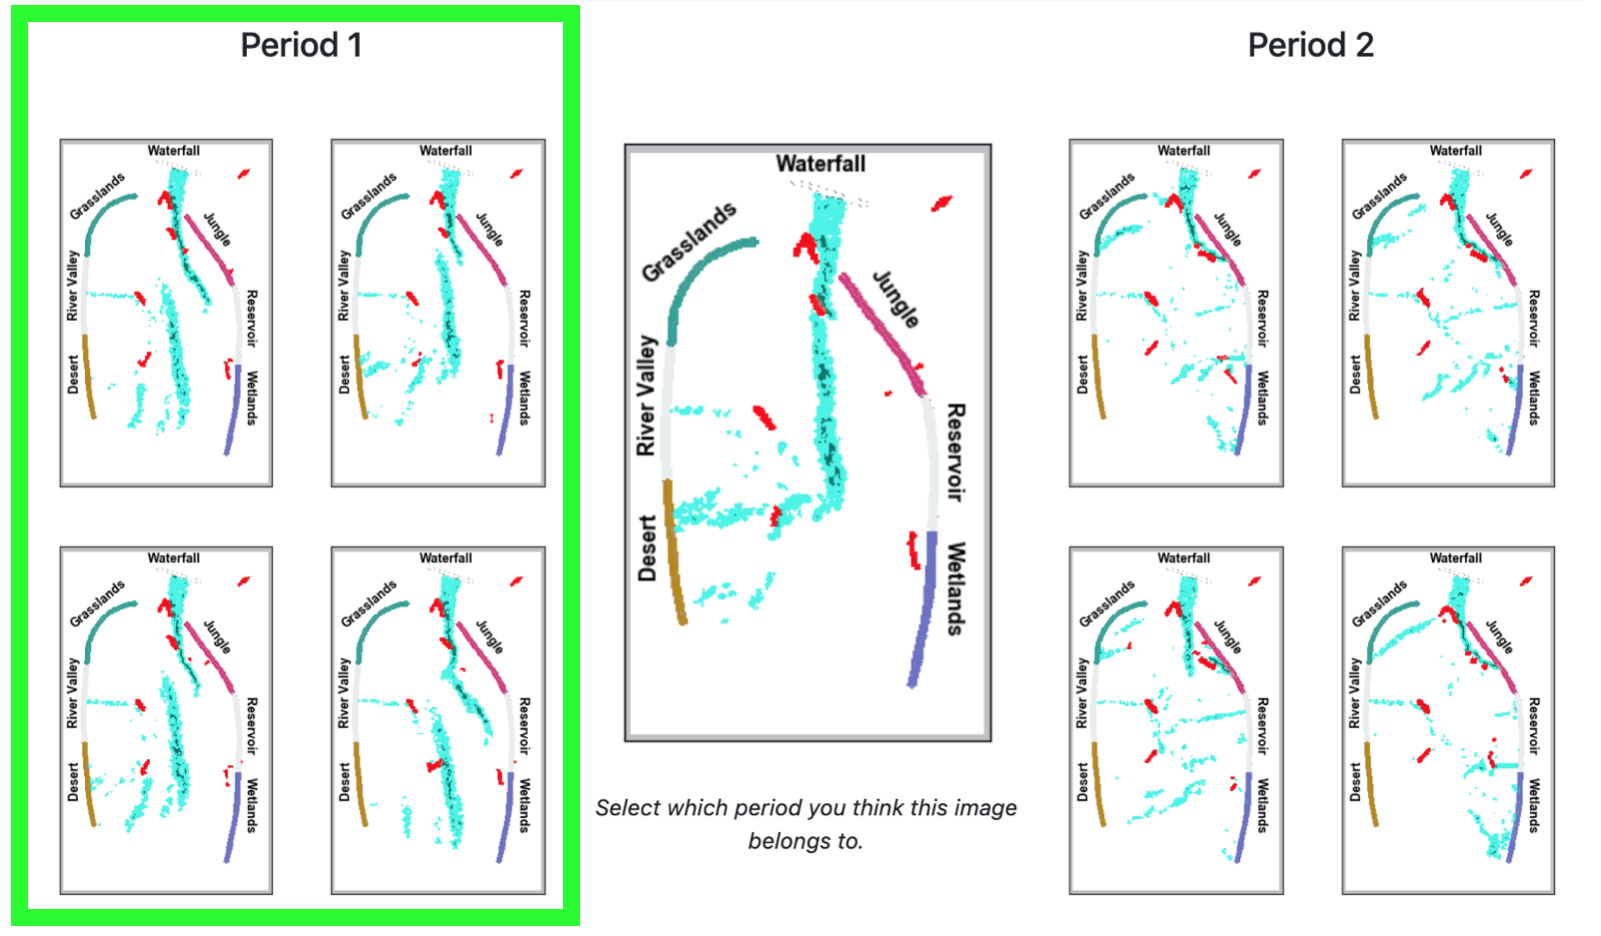
\includegraphics[width=0.70\textwidth]{images/test2_screenshot}
\caption{Screenshot of the  Binary Forced Choice  user interface. An unknown center image needs to be associated with either ``Period 1'' or ``Period 2''. In this case, streams of water flowing to both the Grasslands and to the Jungle capture the dynamics in Period 2. Period 1 has a small amount of water reaching the Desert which is consistent with the unknown image.}
\label{fig:test2_screenshot}
\end{figure*}



















\section{Modeling Students' Activities in CW}
\label{sec:model_for_segmenting_time}

In this section we first describe a general model for segmenting students' activities into periods of time and thereafter present the specific classes of model that are used in our interpretability tests.
The input to the model is the time series that records the levels of water in the different biomes.  The output of a model is a segmentation of the time series   into periods, each of which aims to provide a coherent description of the water flow for a given length of a time.


\subsection{Segmenting Time Series Data into Periods}
Importantly, a single period is insufficient for modeling the effects of students' interactions with CW, because students' sustained actions have complex effects on the system dynamics over time. For example, when students choose to direct water to the Desert and Plains and plant trees in the Desert, the system dynamics are entirely different from the case when water is directed towards the Jungle and the Desert, and the Plains are left to dry. We therefore choose to define multiple periods. Each period describes a length of time where water flowed to a sufficiently stable target according to the model. For example, one period can describe water that mainly flows to the Plains and to the Desert. Students then move logs to re-route water flow to the Jungle, thus starting a new period.

\citename{hoernle2018modeling} used a HMM to model the system responses to the students' activities in CW in which the latent states of the HMM corresponded to periods.
Transitions between different states equates to the system changing between different periods, while self transitions mean the system persists within the same period.
The authors did not address the question of how to choose the number of states. To this end, we augment the HMM with a  hierarchical Dirichlet process which places this non-parametric prior over the state space, following the approach detailed by \citename{teh2005sharing} and \citename{fox2008hdp}.

The ``Sticky-HMM" approach introduced by \citename{fox2008hdp} includes a hyperparameter, $\kappa$, that biases the model to persist in a state, given that it has already adopted that state.
Applied to CW, this parameter can be used to control how much of the water flows are described within each period.
For example, the greater the value for $\kappa$, the more the model will try to persist in any given state.
The increase in the length of periods corresponds to a decrease in the number of latent states.
The opposite is true for lower values of $\kappa$ where there is less bias to persist within a given state and consequently there are more periods that are inferred.
For a detailed description of the model, including the  Gibbs sampling inference scheme that is used to infer the model parameters, please refer to \citename{fox2008hdp,fox2009bayesian}.



\subsection{Model classes}
We introduce three classes of model that segment time into periods that can be used to explain the water flows:

\begin{enumerate}
\item  {${MK_X}$: sticky HMM with fixed $\kappa$.} We use the basic structure of the sticky HMM described by \citename{fox2008hdp} with set values for $\kappa$ to produce $10$ unique models, spanning a wide range of possible settings\footnote{$\kappa \in \{1, 5, 10, 50, 100, 150, 200, 300, 500, 700\}$.}.
\item  {${FB}$: fully Bayesian sticky HMM with Gamma prior on $\kappa$.} This  approach places a weakly informative, conjugate Gamma prior on the hyperparameter that expresses high uncertainty over the $\kappa$ values\footnote{The \textit{(shape,rate)} parameters were chosen to be $(1,\frac{1}{4})$; empirical results were invariant to a range of these values.}.
\item  {${Rand}$: Random baseline.} The random baseline generates periods of random length drawn from a Poisson distribution with mean set to be the mean of all other periods induced by the parametric models. The random periods are defined to include the selected time points ($\{i\}$ from Section~\ref{sec:interpretability_tests}).
\end{enumerate}

\noindent We refer to ${FB}$ as the fully Bayesian model to indicate the fact that the none of the parameters of interest are specified and consequently posterior inference is over all of the parameters in the model (including $\kappa$). This is in contrast to the ${MK_X}$ models where, although these are still Bayesian models, are not fully Bayesian as we explicitly set the value for the sticky parameter $\kappa$.

For models in class $1$ and $2$, we use the Gibbs sampler, described by \citename{fox2008hdp}, to perform inference over the parameters in the model, this includes inference over the state sequence and thus the period segmentation of the model. The observation distribution was chosen to be a mixture of two multivariate Gaussians with conjugate Normal-inverse-Wishart priors. This mixture model addresses the noise in the CW water flow, such as ``splashes'', which prior work has identified as a challenge in this domain~\cite{hoernle2018modeling}.

\section{Model Selection}
\label{sec:model_selection}
The goal of model selection is to optimize a metric such that a specific model architecture with a specific parameter setting can be chosen as the best model for use during inference.
In the absence of performing human interpretability tests, one could choose to optimize some proxy to interpretability~\cite{doshi2017roadmap,lage2018human}. \citename{chang2009reading} compared the proxy of held-out log-likelihood to the human interpretability score that that was a result from two tests that were run on Amazon Mechanical Turk (Mturk).

In a similar manner, we compare the models that are selected by optimizing a human interpretability score  (operationalized as a user  study) to the models that are selected by optimizing statistical information criteria, which are theoretical approximations to using the held-out data in a cross-validation pipeline~\cite{gelman2013bayesian}.
We describe how model selection in these two cases is performed.

\subsection{Selection using an Interpretability Score}

For a given interpretability test $T$,  set of models $\mathcal{M}$, and data set $D$, we aim to find the models that achieve the best interpretability scores ($IS$).

\begin{equation}
\label{eq:model_int_score}
M^*_S \in \argmax_{M \in \mathcal{M}}(IS(M, D))
\end{equation}

Section~\ref{sec:interpretability_results} describes the design and results of a  user study that is
used to find the best model according to the interpretability score.




\subsection{Model Selection using Statistical Theory}
\label{sec:baseline}

Ideally, the model parameters would be optimized on held-out data using predictive log-likelihood as the objective~\cite{chang2009reading}.
However, the difficulty of collecting controlled sessions of student interaction in CW meant we had few data instances available.
To address this challenge we use  statistical information criteria as a theoretical approximation to the predictive accuracy of a model~\cite{gelman2013bayesian}. Specifically, we use the following information criteria:
the {Deviance Information Criterion (DIC)} and {Watanabe-Akaike Information Criterion (WAIC)}.






Let $ \log P( D \mid \hat{M} )$ be the log-likelihood of the data given a model $\hat{M}$ with parameters set to the mean of the posterior estimates. The DIC is defined as follows:
\begin{equation}
\label{eq:dic_formula}
DIC (M, D) = -2 \log p(D \mid \hat{M}) + 2\cdot c_1
\end{equation}
where $c_1$ is a penalization term\footnote{Exact formulae for the DIC and WAIC penalization terms can be found in \citename{gelman2013bayesian} in the section starting at pg.169.} that depends on
the expectation of the log-likelihood of the data given $M$.  In practice, this expectation is the average of $\log P(D\mid M)$, where $M$ corresponds to parameters that are obtained via the posterior distribution samples from the Gibbs sampler.

The WAIC has the same structure, although it does not require $\hat{M}$:
\begin{equation}
\label{eq:waic_formula}
WAIC (M ,D) = - 2 \log E[ P( D \mid M ) ] + 2c_2
\end{equation}

\noindent here, the penalising factor $c_2$
subtracts $E[ \log P (D \mid M )]$ from $\log\left( E[ P ( D \mid M )]\right)$.
Again, these expectations are computed using Monte Carlo estimates from the individual posterior samples from the Gibbs sampler.

Model selection is performed by assigning $IC$ to be $WAIC$ or $DIC$ respectively and minimizing Equation~\ref{eq:model_information_criteria}.
\begin{equation}
\label{eq:model_information_criteria}
M^*_C \in \argmin_{M \in \mathcal{M}}(IC(M, D))
\end{equation}

Figure~\ref{fig:dic_waic_scores} shows the two information criteria plotted as a function of the model (the random model has no notion of information criteria and so was not compared here). The data set comprised of both of the log files of students' interactions (8 minutes each). The optimal model for both DIC and WAIC is the $MK_{5}$ model but we note that $MK_{1}$, $MK_{5}$ and $MK_{10}$ all perform close to this optimal setting. Notice that the fully Bayesian model (FB) is not optimal but it is in the top $5$ models for both criteria.
\begin{figure}[t]
\centering
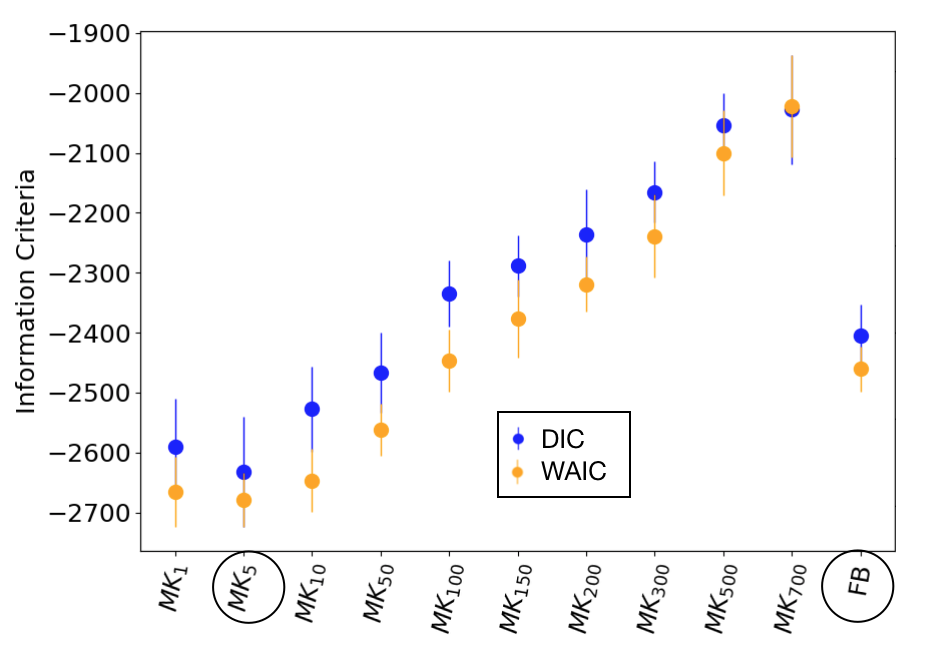
\includegraphics[width=0.48\textwidth]{images/dic_waic_scores.png}
\caption{DIC and WAIC as a function of the model (lower on y-axis is better). The $MK_5$ model is optimal, the $FB$ approach is in 5th place.}
\label{fig:dic_waic_scores}
\end{figure}











\section{User Study}
\label{sec:interpretability_results}



In this section we describe a user study that compares the interpretability of different models for describing the responses of the simulation to students' interactions in CW.
The set of models includes the 12 CW models described in Section~\ref{sec:model_for_segmenting_time}.%; a time series $D$ consists of an 8-minute interaction sequence of students' activities.









We recruited participants from two cohorts: undergraduate engineering students in a large public university
and Mturk workers (with a total of $240$ people who participated in the experimentation).
For a given data instance, we randomly sampled a set of 12 time points, which  remained constant across all model conditions.
Each time point generated 2 experiment trials for each model, making $2 \times 12 \times 12=288$ trials per data instance. The reason for $2$ trials per time point is to select both the forward and backward intruders (in time) for each selected candidate period. Each participant saw 20 randomly sampled experiment trials, with no more than 2 trials from any given model, to ensure a representative range of models.
After making their choice, participants received brief visual feedback on whether or not their selection was correct.

All participants received a detailed tutorial about CW and the study, as well as a pre-study comprehension quiz\footnote{Tutorial pdf slides are available in the supplementary material.}. Mturk workers were paid a base rate of $\$0.25$ for participating and a bonus structure of $\$0.1$ for each correct response.






\begin{figure}[t]


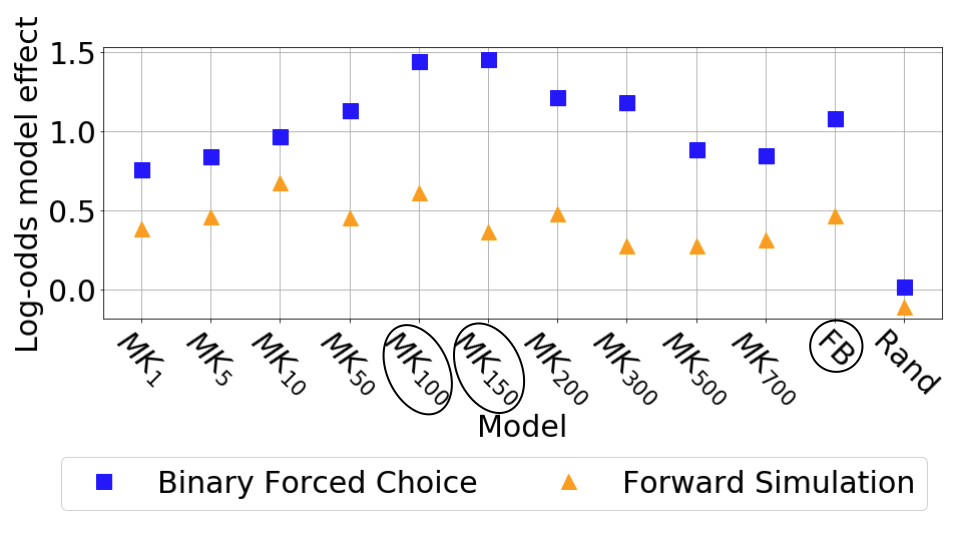
\includegraphics[width=.48\textwidth]{images/combined_res_data_all.png}
\caption{Effect of each model on the log-odds of a test evaluator selecting the correct response (controlling for the test evaluator, the experiment trial, log file and ordering effects).}
\label{fig:essil_test_results}
\end{figure}


We first describe results in terms of accuracy (the percent of correctly labelled test instances).
The top performing model was $MK_{200}$ with an accuracy of $83\%$ on the Forward Simulation  test and $MK_{100}$  with an accuracy of $82\%$ on the Binary Forced Choice test.
The random baseline model performed consistently poorly with an average accuracy of $53\%$ on both tests.
The fully Bayesian model achieved an accuracy of $72\%$ and $70\%$ respectively on the two tests.

\vspace{-1.60mm}
To control for ordering effects, chosen time periods, data instance used, and effects of individual participants, we applied an L2 regularized logistic regression for predicting  the user specific success on the experiment trial, shown  in  Figure~\ref{fig:essil_test_results}. The y-axis presents the improvement in log-odds that a model has on the expected response accuracy (higher is better).
As shown by the figure,  the Forward Simulation shows a high variance with no clear maximum. In contrast, the Binary Forced Choice test has a clear maximum in the region of $MK_{100}$ and $MK_{150}$.  From both Figures~\ref{fig:dic_waic_scores} and~\ref{fig:essil_test_results} we can infer the following four conclusions.
First, all of the models ($MK_{1},\ldots,MK_{700}, FB$) outperform the random baseline: participants are more likely to select the correct response from any of these models. This result suggests that periods of stable dynamics  exist in the data and that it is possible to construct models, which describe these dynamics, that are interpretable to people.  Second, the Binary Forced Choice test is a preferable measure for interpretablity   to the Forward Simulation test. Figure~\ref{fig:essil_test_results} shows that the Binary Forced Choice test exhibits a clear peak (around $MK_{100}$ and $MK_{150}$) where interpretability of the model is maximized.
These models also maximized the  raw accuracy on the Binary Forced Choice test.

On the other hand, the Forward Simulation test has a greater variance across models and across data instances.
Two possible causes for this higher variance are: (1) there is more room for error in the Forward Simulation test (5 choices vs. 2 choices in Binary Forced Choice); (2) sampling a single image to represent a period (as in Forward Simulation) presents less information to the user than sampling 4 images (as in Binary Forced Choice).

Third, the best $\kappa$ settings vary for different tests and information criteria.
Model interpretability grows steadily as the value of $\kappa$ increases, with $MK_{100}$ and $MK_{150}$ being the optimal models, and then proceeds to decrease steadily.
These models are not consistent with the model $MK_5$ that optimized the information criteria.
Note that higher $\kappa$ values are ``sticky'' - they  bias the model towards longer periods, which condense too many activities to make sense to people.
On the other end of the spectrum, lower $\kappa$ values allow for shorter periods that capture too much of the noise in the system.
In contrast, the $\kappa$ value for  models $MK_{100}$ and $MK_{150}$
represent a ``sweet spot" in between these two extremes.


Finally, the fully Bayesian model $(FB)$ performs consistently well on both information criteria and interpretability tests. It is interesting to note that while this model does not find the optimal setting (from neither the statistical information criteria nor from the human interpretability task) it does perform well across all tests, tasks and instances, and is fully automated (no human evaluation is required in order to choose an optimal parameter setting).

We conclude this section with mentioning the limitation that the user study was based on a small number $(n=2)$  of instances. This was due to the difficulty in obtaining controlled sessions of student behavior in CW. Despite this issue, the differences between the models in Figure~\ref{fig:essil_test_results} are statistically significant, having being evaluated across 12 different time points for each instance and with hundreds of evaluators.

























\vspace{-1.51mm}
\section{Conclusion \& Future Work}


With the growing prevalence of immersive simulations so arises the need for AI systems which help end-users gain insight into the activities of the participants.
We have studied an environmental simulation where students learn about the causal effects of their actions.
Our results show that algorithms can segment time series log data into periods that are coherent for people.
However, selecting hyperparameters in these models is a challenge, especially when trying to optimize the representations for their interpretability.
We have shown an example of how to select these hyperparameters from two tests that are grounded in the literature and we have further presented the fully Bayesian method as promising technique for implementing a model when human evaluations are not possible.
Future work will apply these models to alternative domains and will work with teachers and experts ``in the loop'' such that we can target the goal of engaging the participants with insights drawn from their own experiences with such immersive simulations.

\bibliographystyle{aaai.bst}
Modi itaque veniam, magni rem quis ipsa qui veniam voluptate, illo eum laudantium praesentium cumque repellat nemo animi minus obcaecati, minima perferendis fuga illum aspernatur sequi praesentium?Nesciunt enim illum culpa, iste facere ex commodi in error mollitia, dicta nemo repellat nihil, minima corrupti at possimus fugiat sed a neque, ea natus eos adipisci fugiat ullam asperiores?Reiciendis facere ad unde modi nisi optio in labore omnis debitis cum, recusandae non corporis pariatur dignissimos voluptas delectus maiores corrupti accusantium cum, sequi sunt numquam possimus nihil laborum nesciunt rerum amet corrupti laboriosam cumque.Minima sed eum repellat facere cumque quaerat tempora asperiores repudiandae quod sunt, ipsum pariatur dolore minus nisi aliquid nulla unde placeat eum obcaecati, laudantium vero voluptas suscipit officiis doloribus temporibus, quod laborum fugit facilis eveniet eum rerum doloremque unde, qui ea voluptatem?Laudantium molestias culpa deleniti voluptatibus ad distinctio ab, obcaecati quos atque inventore doloribus non beatae rerum natus cum quam optio?Ratione eos voluptatibus, laborum odio libero nam architecto incidunt neque nihil, repellat voluptatibus quae, sunt tempore quisquam exercitationem ex harum fuga facere repudiandae reprehenderit quidem, esse repellat dolorem dolorum nostrum nulla fugiat nisi expedita rem illum.\clearpage
\bibliography{bibliography}
\end{document}










